
\documentclass{standalone}
\usepackage{tikz}

\begin{document}
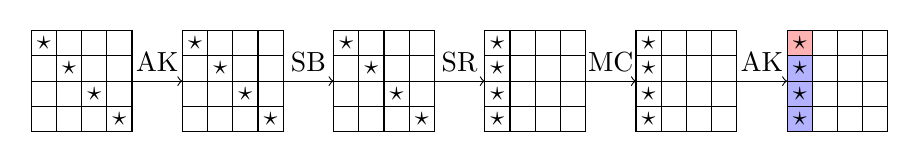
\begin{tikzpicture}[scale=0.32]

  % Title
  % \node at (13, 24) {\Large\textbf{4-Round Diagonal Integral Distinguisher}};

  % ========== Plaintext ==========
  \begin{scope}[yshift=0cm,xshift=-6cm]
    \path[shift={(0.5,0.5)}] (0,3) node {$\star$};
    \path[shift={(0.5,0.5)}] (1,2) node {$\star$};
    \path[shift={(0.5,0.5)}] (2,1) node {$\star$};
    \path[shift={(0.5,0.5)}] (3,0) node {$\star$};
    \draw (0,0) rectangle (4,4);
    \draw (0,1) -- +(4,0);
    \draw (0,2) -- +(4,0);
    \draw (0,3) -- +(4,0);
    \draw (1,0) -- +(0,4);
    \draw (2,0) -- +(0,4);
    \draw (3,0) -- +(0,4);
    % \path (6,2) node {diagonal $\delta$-set};
    % \draw (0,2) -- ++(-1.5,0) -- +(0,-24.4);
    \draw[->] (4,2)-- node[above]{AK} ++(2,0);
  \end{scope}

    \begin{scope}[yshift=0cm,xshift=0cm]
    \path[shift={(0.5,0.5)}] (0,3) node {$\star$};
    \path[shift={(0.5,0.5)}] (1,2) node {$\star$};
    \path[shift={(0.5,0.5)}] (2,1) node {$\star$};
    \path[shift={(0.5,0.5)}] (3,0) node {$\star$};
    \draw (0,0) rectangle (4,4);
    \draw (0,1) -- +(4,0);
    \draw (0,2) -- +(4,0);
    \draw (0,3) -- +(4,0);
    \draw (1,0) -- +(0,4);
    \draw (2,0) -- +(0,4);
    \draw (3,0) -- +(0,4);
    % \path (6,2) node {diagonal $\delta$-set};
    % \draw (0,2) -- ++(-1.5,0) -- +(0,-24.4);
        \draw[->] (4,2)-- node[above]{SB} ++(2,0);
  \end{scope}

      \begin{scope}[yshift=0cm,xshift=6cm]
    \path[shift={(0.5,0.5)}] (0,3) node {$\star$};
    \path[shift={(0.5,0.5)}] (1,2) node {$\star$};
    \path[shift={(0.5,0.5)}] (2,1) node {$\star$};
    \path[shift={(0.5,0.5)}] (3,0) node {$\star$};
    \draw (0,0) rectangle (4,4);
    \draw (0,1) -- +(4,0);
    \draw (0,2) -- +(4,0);
    \draw (0,3) -- +(4,0);
    \draw (1,0) -- +(0,4);
    \draw (2,0) -- +(0,4);
    \draw (3,0) -- +(0,4);
    % \path (6,2) node {diagonal $\delta$-set};
    % \draw (0,2) -- ++(-1.5,0) -- +(0,-24.4);
        \draw[->] (4,2)-- node[above]{SR} ++(2,0);
  \end{scope}


      \begin{scope}[yshift=0cm,xshift=12cm]
    \path[shift={(0.5,0.5)}] (0,3) node {$\star$};
    \path[shift={(0.5,0.5)}] (0,2) node {$\star$};
    \path[shift={(0.5,0.5)}] (0,1) node {$\star$};
    \path[shift={(0.5,0.5)}] (0,0) node {$\star$};
    \draw (0,0) rectangle (4,4);
    \draw (0,1) -- +(4,0);
    \draw (0,2) -- +(4,0);
    \draw (0,3) -- +(4,0);
    \draw (1,0) -- +(0,4);
    \draw (2,0) -- +(0,4);
    \draw (3,0) -- +(0,4);
    % \path (6,2) node {diagonal $\delta$-set};
    % \draw (0,2) -- ++(-1.5,0) -- +(0,-24.4);
        \draw[->] (4,2)-- node[above]{MC} ++(2,0);
  \end{scope}

        \begin{scope}[yshift=0cm,xshift=18cm]
    \path[shift={(0.5,0.5)}] (0,3) node {$\star$};
    \path[shift={(0.5,0.5)}] (0,2) node {$\star$};
    \path[shift={(0.5,0.5)}] (0,1) node {$\star$};
    \path[shift={(0.5,0.5)}] (0,0) node {$\star$};
    \draw (0,0) rectangle (4,4);
    \draw (0,1) -- +(4,0);
    \draw (0,2) -- +(4,0);
    \draw (0,3) -- +(4,0);
    \draw (1,0) -- +(0,4);
    \draw (2,0) -- +(0,4);
    \draw (3,0) -- +(0,4);
    % \path (6,2) node {diagonal $\delta$-set};
    % \draw (0,2) -- ++(-1.5,0) -- +(0,-24.4);
        \draw[->] (4,2)-- node[above]{AK} ++(2,0);
  \end{scope}


        \begin{scope}[yshift=0cm,xshift=24cm]
          \fill[red!30] (0,3) rectangle ++(1,1);
                  \fill[blue!30] (0,0) rectangle ++(1,3);
    \path[shift={(0.5,0.5)}] (0,3) node {$\star$};
    \path[shift={(0.5,0.5)}] (0,2) node {$\star$};
    \path[shift={(0.5,0.5)}] (0,1) node {$\star$};
    \path[shift={(0.5,0.5)}] (0,0) node {$\star$};
    \draw (0,0) rectangle (4,4);
    \draw (0,1) -- +(4,0);
    \draw (0,2) -- +(4,0);
    \draw (0,3) -- +(4,0);
    \draw (1,0) -- +(0,4);
    \draw (2,0) -- +(0,4);
    \draw (3,0) -- +(0,4);


    % \path (6,2) node {diagonal $\delta$-set};
    % \draw (0,2) -- ++(-1.5,0) -- +(0,-24.4);
        % \draw[->] (4,2)-- node[above]{AK} ++(2,0);
  \end{scope}
  

\end{tikzpicture}
\end{document}
